\documentclass{article}
\usepackage[utf8]{inputenc}
\usepackage{graphicx}
\usepackage[spanish]{babel}
\usepackage{siunitx}
\usepackage{url}
\usepackage{float}
\usepackage[table,xcdraw]{xcolor}
\usepackage{multirow}
\setlength\parindent{0pt}
\tolerance=9999
\hyphenpenalty=10000
\exhyphenpenalty=100
\graphicspath{ {./images/} }

\begin{document}

\begin{titlepage}
    \begin{center}
        \large    
        
        Milagros Bello, Pilar Castroman, Ailen Valli,
        
        Camila Vázquez, Matias Vicente y Guillermo Wajner
        
        \vspace{6cm}
        \Huge
        \textbf{Ensayo a la Llama}

        \vspace{0.5cm}

        \Large
        12 de mayo de 2022

        \vspace{6cm}
        
        \normalsize
        5\textsuperscript{o} Biológico y Científico\\
        St. George’s Secondary School\\
        Química\\
        Prof. Cecilia Saettone
        \vspace{0.5cm}      
    \end{center}
\end{titlepage}

\section{Objetivo}

El objetivo de la práctica radica en observar e interpretar los cambios cromáticos producidos en una llama al momento de calentar diferentes sustancias.  

\section{Fundamento Teórico}

El ensayo a la llama es una técnica utilizada para identificar determinadas sustancias por medio de su composición cualitativa. El mismo se trata de someter una muestra al calor y apreciar los diferentes colores que identifican a cada elemento presente en dicha muestra.\\

Al absorber energía los átomos alcanzan un estado excitado, por lo que tienden a volver a su estado fundamental. Para esto deben perder energía. El estado fundamental es igual para todos los átomos. Por el contrario, los estados excitados son particulares para cada elemento, lo que implica que la radiación emitida también será particular para cada elemento. A partir de esto es posible decir que la radiación nos permite poder identificar a un elemento. A la hora de calentar un metal o sus compuestos estos adquieren un color que identifica a cada elemento metálico.\\

A continuación, el cuadro 1 muestra algunos elementos metálicos y el color de la llama que le corresponde a cada elemento una vez que la sustancia correspondiente entra en contacto con ella. A su vez, se determina la intensidad del mismo. 

\begin{table}[H]
\centering
\begin{tabular}{|l|l|l|}
\hline
\rowcolor[HTML]{C0C0C0} 
\multicolumn{1}{|c|}{\cellcolor[HTML]{C0C0C0}Elemento Metálico} & \multicolumn{1}{c|}{\cellcolor[HTML]{C0C0C0}Color de la llama} & \multicolumn{1}{c|}{\cellcolor[HTML]{C0C0C0}Intensidad} \\ \hline
Litio (Li) & Rojo & Alta \\ \hline
Sodio (Na) & Amarillo & Muy Alta \\ \hline
Potasio (K) & Violeta & Alta \\ \hline
Calcio (Ca) & Rojo-Anaranjado & Media \\ \hline
Estroncio (Sr) & Rojo & Media \\ \hline
Bario (Ba) & Verde claro & Baja \\ \hline
\end{tabular}
\caption{intensidad y color de llama para elementos metálicos}
\label{table:elem}
\end{table}

\section{Materiales}

\begin{itemize}
    \item Fósforo
    \item Espátulas
    \item Sales
    \item Etanol
    \item Mechero
\end{itemize}

\section{Sustancias y Mezclas}

\begin{table}[H]
\begin{tabular}{|r|l|}
\hline
\rowcolor[HTML]{C0C0C0} 
\multicolumn{1}{|l|}{\cellcolor[HTML]{C0C0C0}Fórmula} & Nombre de la Sal \\ \hline
\rowcolor[HTML]{FFFFFF} 
KI & \cellcolor[HTML]{FFFFFF}Yoduro de Potasio \\ \hline
\cellcolor[HTML]{FFFFFF}K\textsubscript{2}SO\textsubscript{4} & Sulfato de Potasio \\ \hline
\cellcolor[HTML]{FFFFFF}NaCl & Cloruro de Sodio \\ \hline
\cellcolor[HTML]{FFFFFF}Na\textsubscript{2}SO\textsubscript{4} & Sulfato de Sodio \\ \hline
\cellcolor[HTML]{FFFFFF}CuCl & Cloruro Cuproso \\ \hline
\cellcolor[HTML]{FFFFFF}CuCl\textsubscript{2} & Cloruro Cúprico \\ \hline
Sr(NO\textsubscript{3})\textsubscript{2} & Nitrato de Estroncio \\ \hline
\cellcolor[HTML]{FFFFFF}SrCl\textsubscript{2} & Cloruro de Estroncio \\ \hline
\end{tabular}
\end{table}

\section{Datos de Seguridad}

\begin{figure}[H]
    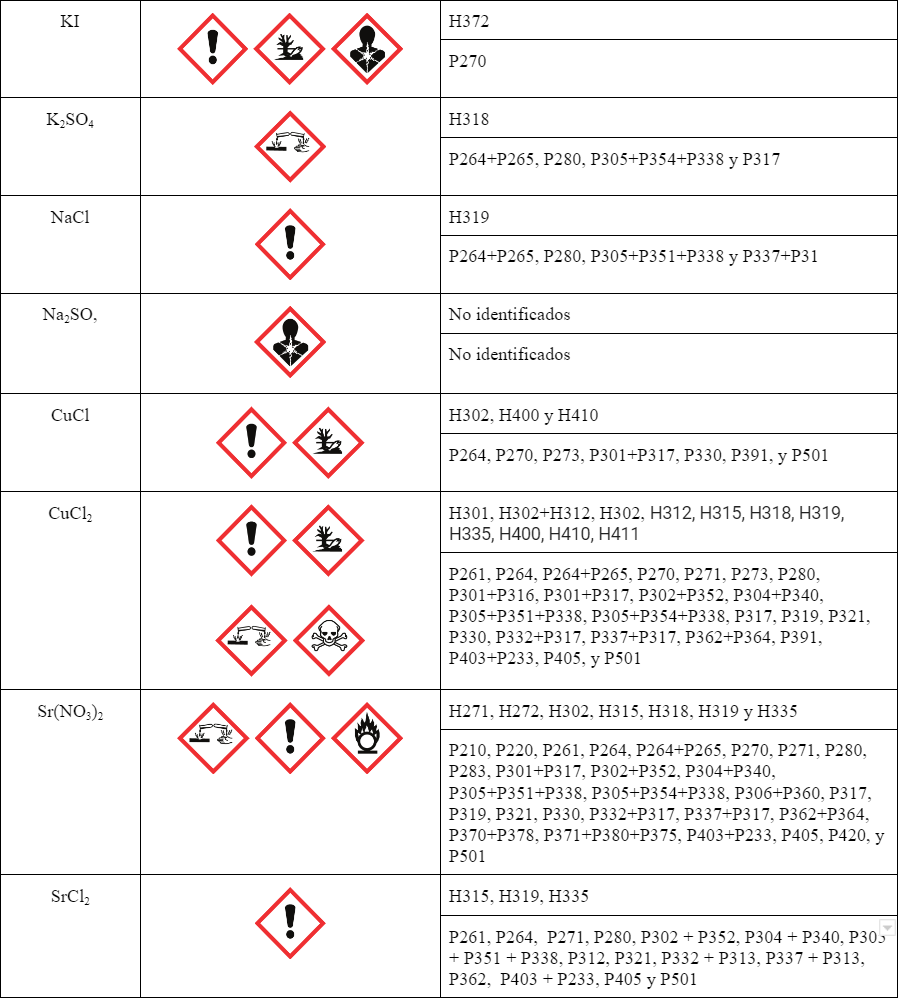
\includegraphics[width=0.9\textwidth]{seguridad.png}
    \label{fig:hazard}
\end{figure}

\section{Procedimiento}

\begin{enumerate}
  \item Encender el mechero.
  \item Tomar con la espátula una muestra de una de las sales.
  \item Insertarla en la llama.
  \item Observar el color de la llama.
  \item Repetir el mismo procedimiento para todas las sustancias.

\end{enumerate}

\section{Procesamiento y Sistematización de Datos Experimentales}

\begin{table}[H]
\begin{tabular}{|l|l|l|}
\hline
\rowcolor[HTML]{D9D9D9} 
Sustancia & Catión metálico & Color de la llama \\ \hline
\cellcolor[HTML]{FFFFFF}KI & K\textsuperscript{+} & Rosado \\ \hline
K\textsubscript{2}SO\textsubscript{4} & K\textsuperscript{+} & Rosado \\ \hline
NaCl & Na\textsuperscript{+} & Amarillo \\ \hline
Na\textsubscript{2}SO\textsubscript{4} & Na\textsuperscript{+} & Amarillo \\ \hline
CuCl & Cu\textsuperscript{+} & Verde \\ \hline
CuCl\textsubscript{2} & Cu\textsuperscript{2+} & Verde \\ \hline
Sr(NO\textsubscript{3})\textsubscript{2} & Sr\textsuperscript{2+} & Rojo \\ \hline
SrCl\textsubscript{2} & Sr\textsuperscript{2+} & Rojo \\ \hline
\end{tabular}
\end{table}

\section{Interpretación y Discusión de Resultados Experimentales}

El color que se observa en la llama corresponde a la longitud de onda del momento en que los electrones bajan de nivel de energía.\\

Este método de identificación de la composición cualitativa presenta ventajas y desventajas. El mismo nos permite restringir la cantidad de posibilidades a la hora de identificar una sustancia, sin embargo, el color que se muestra en la práctica al momento de llevarla a cabo corresponde al catión que conforma a la sustancia y no a la sustancia propiamente dicha.  


\pagebreak

\section{Referencias Bibliográficas}

Saettone, C. (2022) \textit{Química Práctico Quinto Año 2022}\\

National Center for Biotechnology Information (2022 a). \textit{PubChem Compound Summary for CID 4875, Potassium iodide.} Recuperado el 18 de mayo de 2022 de \url{https://pubchem.ncbi.nlm.nih.gov/compound/Potassium-iodide}.\\

National Center for Biotechnology Information (2022 b). \textit{PubChem Compound Summary for CID 24507, Potassium sulfate.} Recuperado el 18 de mayo de 2022 de \url{https://pubchem.ncbi.nlm.nih.gov/compound/Potassium-sulfate}.\\

National Center for Biotechnology Information (2022 c). \textit{PubChem Compound Summary for CID 5234, Sodium chloride.} Recuperado el 18 de mayo de 2022 de \url{https://pubchem.ncbi.nlm.nih.gov/compound/Sodium-chloride}.\\

National Center for Biotechnology Information (2022 d). \textit{PubChem Compound Summary for CID 24436, Sodium sulfate.} Recuperado el 18 de mayo de 2022 de \url{https://pubchem.ncbi.nlm.nih.gov/compound/Sodium-sulfate}.\\

National Center for Biotechnology Information (2022 e). \textit{PubChem Compound Summary for CID 62652, Copper(I) chloride.} Recuperado el 18 de mayo de 2022 de \url{https://pubchem.ncbi.nlm.nih.gov/compound/Copper_I_-chloride}.\\

National Center for Biotechnology Information (2022 f). \textit{PubChem Compound Summary for CID 24014, Cupric chloride.} Recuperado el 18 de mayo de 2022 de \url{https://pubchem.ncbi.nlm.nih.gov/compound/Cupric-chloride}.\\

National Center for Biotechnology Information (2022 g). \textit{PubChem Compound Summary for CID 24848, Strontium nitrate.} Recuperado el 18 de mayo de 2022 de \url{https://pubchem.ncbi.nlm.nih.gov/compound/Strontium-nitrate}.\\

National Center for Biotechnology Information (2022 h). \textit{PubChem Compound Summary for CID 61520, Strontium chloride (SrCl2).} Recuperado el 18 de mayo de 2022 de \url{https://pubchem.ncbi.nlm.nih.gov/compound/Strontium-chloride-_SrCl2}.\\

\end{document}
